%!TEX root = ../report.tex

\begin{document}
    \chapter{Datasets and Benchmarking}
    \section{Semantic3D}
Semantic3D is a huge 3D benchmark point cloud classification dataset and classified as static dataset.
The dataset consists of nearly 4 billion points which contain variety of scenes in urban and rural setting.
These scenes are taken in places such as markets, dom, stations and fields collected in European streets with terrestrial lasers.
Each point in the point cloud consists of geometric positions (x, y, and z), color (R, G, and B) and intensity values as features.
Example point cloud scenes are provided in Figure \ref{fig:sem3d_gt_vis}. 

The dataset consits of 8 classes and they include
\begin{enumerate}
    \item man-made terrain - pavement
    \item natural terrain - grass
    \item high vegetation - large bushes and trees
    \item low vegetation - flowers and bushes less than 2cm in height
    \item buildings - stations, churches, cityhalls
    \item hardscapes - garden walls, banks, fountains
    \item scanning artificats - dynmically moving objects
    \item cars
\end{enumerate}
The distribution of these calsses are given in Figure \ref{fig:sem3ddist}.
From this graph, we can observe that the manmade terrain made most of the dataset because the lidar is placed on street during collection.
As they are near to lidar and it is common with outdoor lidar datasets.
The classes low vegetation, hardscapes, scanning artificats and cars have less number of training points and lower performance from the model on these classes are to be expected.
Also according to \cite{hackel2017semantic3d}, scanning artifacts, cars and hardscapes are toughest classes becuase of variation in obejct shapes.
\cite{survey3d} also proves that the Semantic3D is most diverse dataset in 3D LiDAR data compared to other datasets such as SemanticKITTI and SemanticPOSS.
Becuase of these reasons, we considered using Semantic3D dataset as in distribution training data.
The dataset is available to download on http://www.semantic3d.net/. 
As this is an ongoing benchmark challenge, the labels for the testing data is not available.
We made use of validation set for evaluation purpose which is a subset of trianing set.
\begin{figure}[h!]
    \centering
    \includestandalone[width=0.6\linewidth]{images/Sem3d_points}
    \caption{Distribution of training points in million per class in Semantic3D dataset. \textcolor{red}{Make it log scale}}
    \label{fig:sem3ddist}
\end{figure}


%        
\includegraphics[scale=0.55]{images/legend.png}    
\begin{figure*}
    \centering
    \begin{tabular}{cc}
        RGB & Ground truth \\
        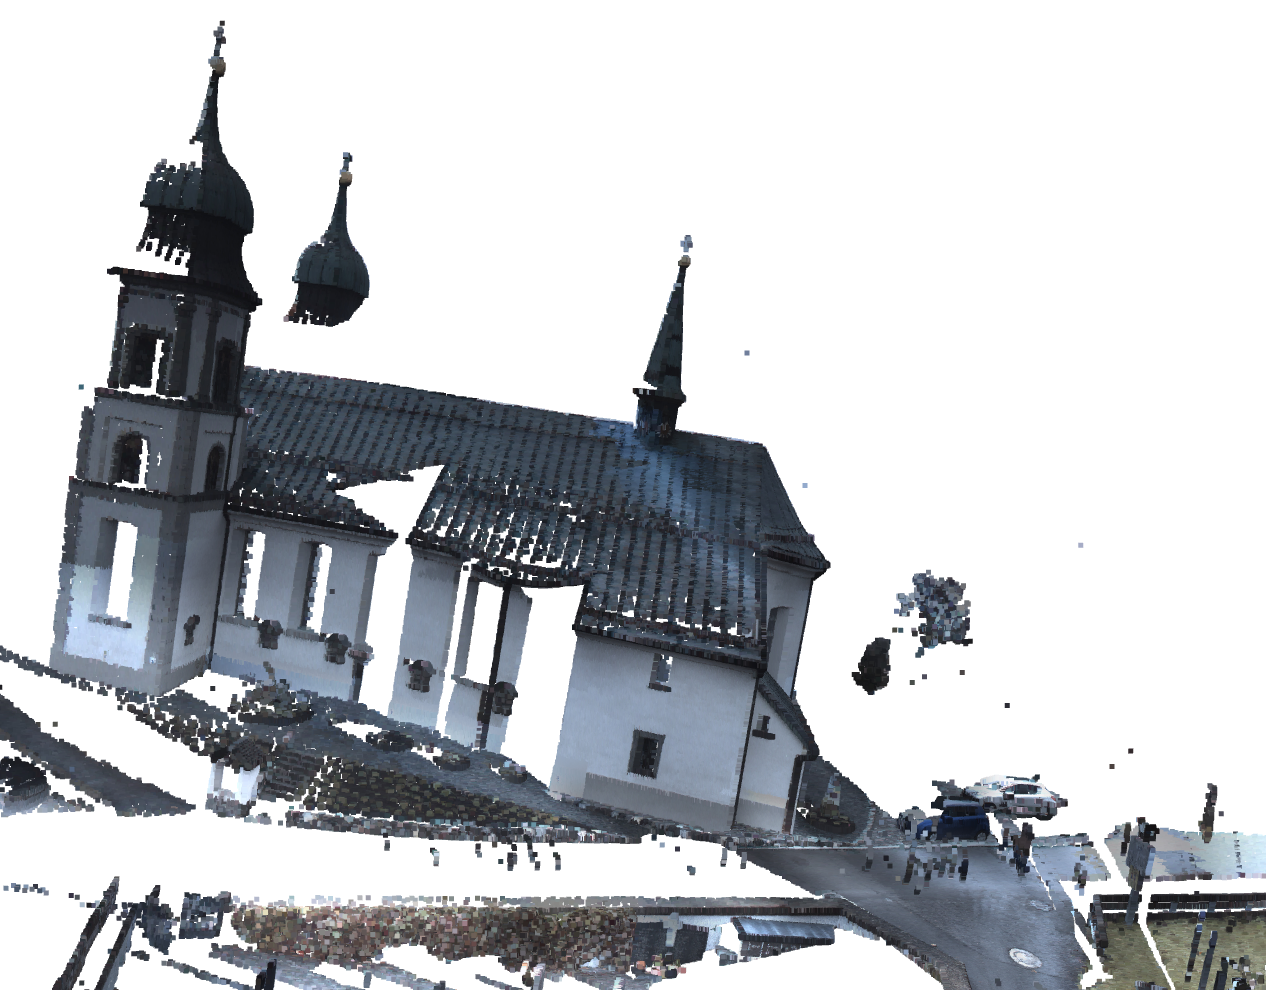
\includegraphics[width=0.35\textwidth, height=0.15\textheight]{images/sem3d_data/1.png} & 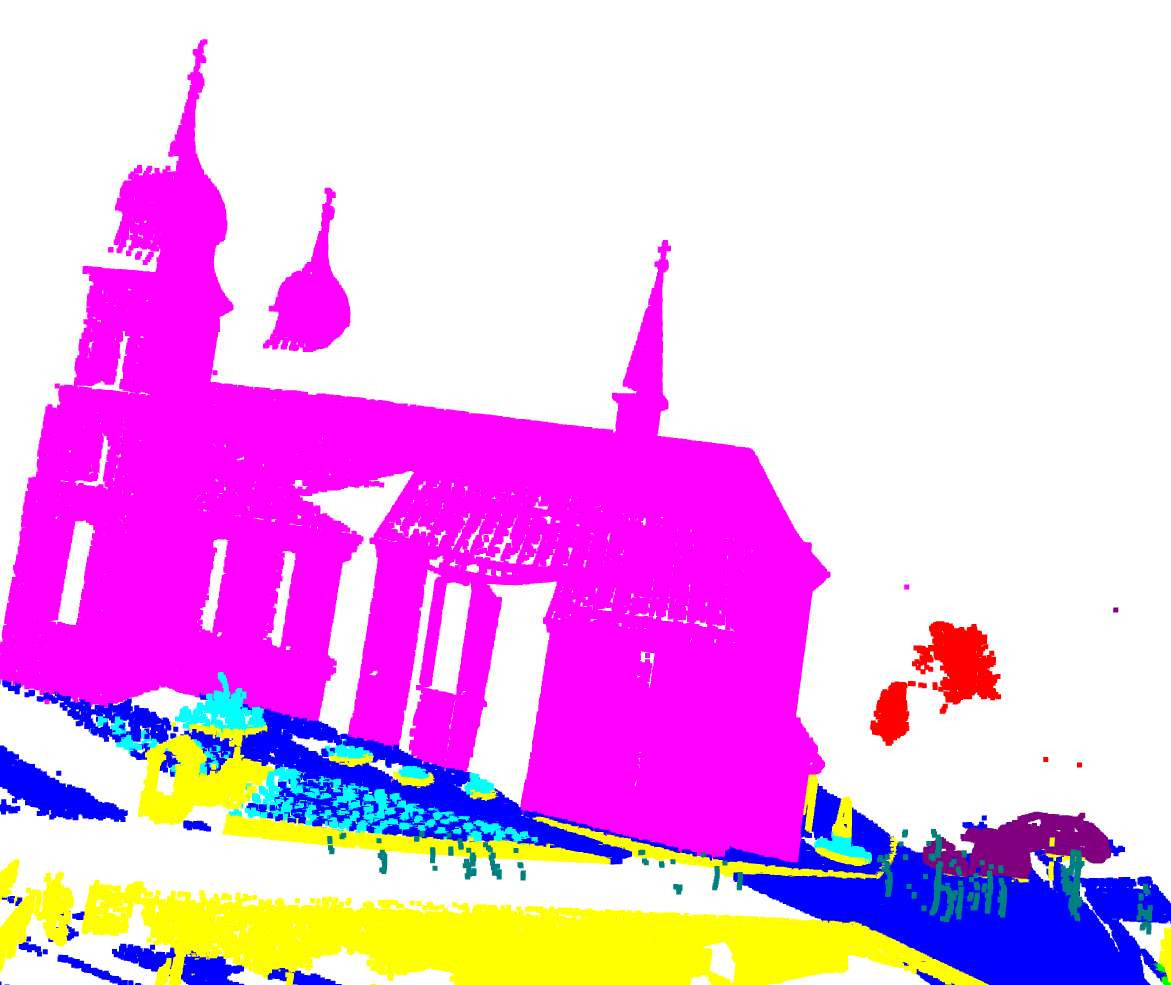
\includegraphics[width=0.35\textwidth, height=0.15\textheight]{images/sem3d_data/1_gt.png}\\
        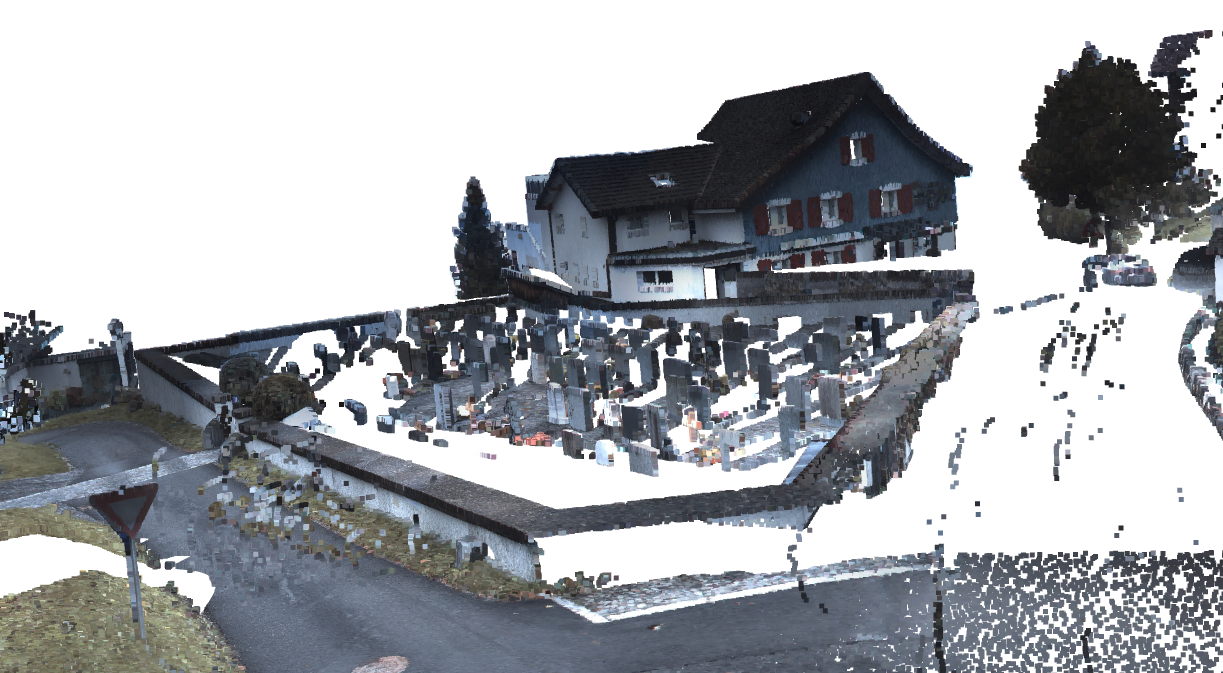
\includegraphics[width=0.35\textwidth, height=0.15\textheight]{images/sem3d_data/2.png} & 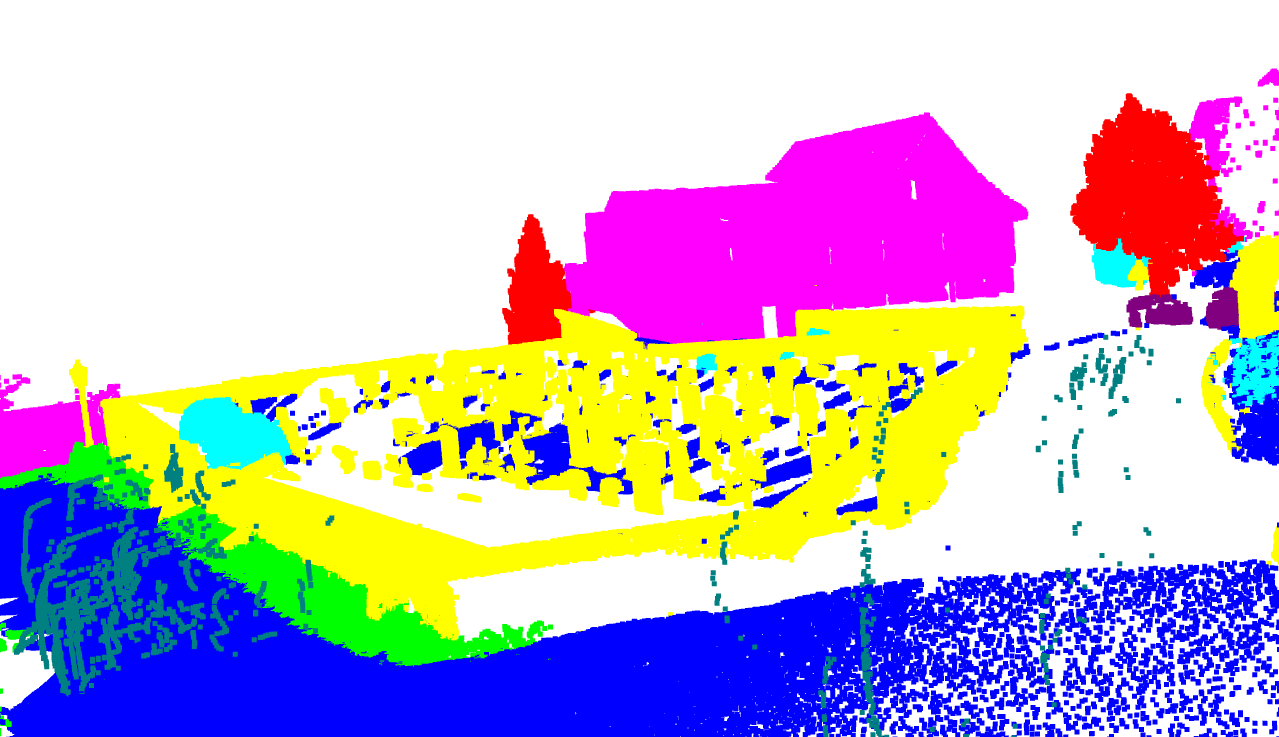
\includegraphics[width=0.35\textwidth, height=0.15\textheight]{images/sem3d_data/2_gt.png}\\
        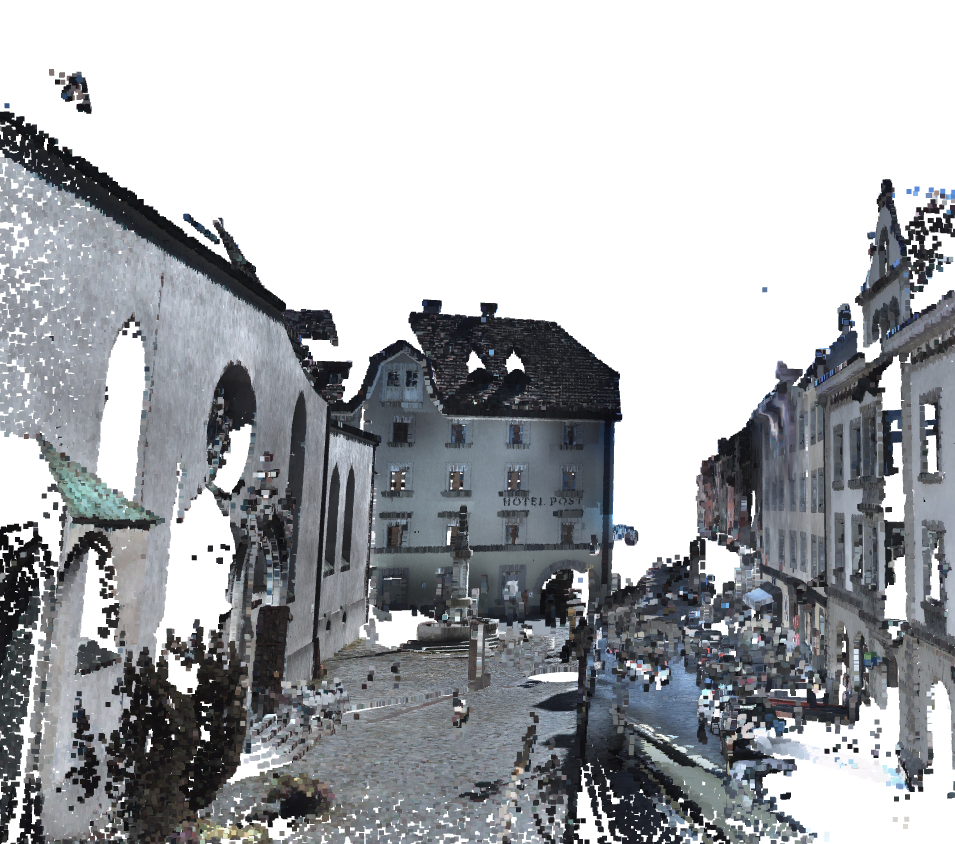
\includegraphics[width=0.35\textwidth, height=0.15\textheight]{images/sem3d_data/3.png} & 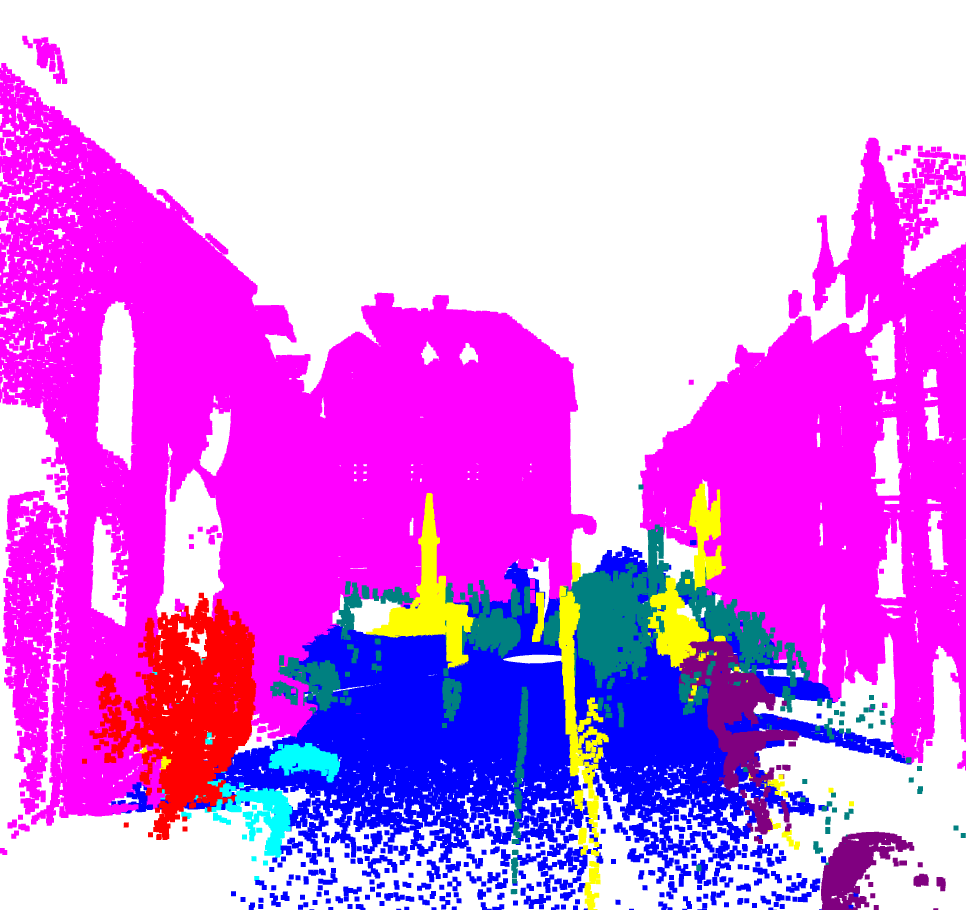
\includegraphics[width=0.35\textwidth, height=0.15\textheight]{images/sem3d_data/3_gt.png}\\
        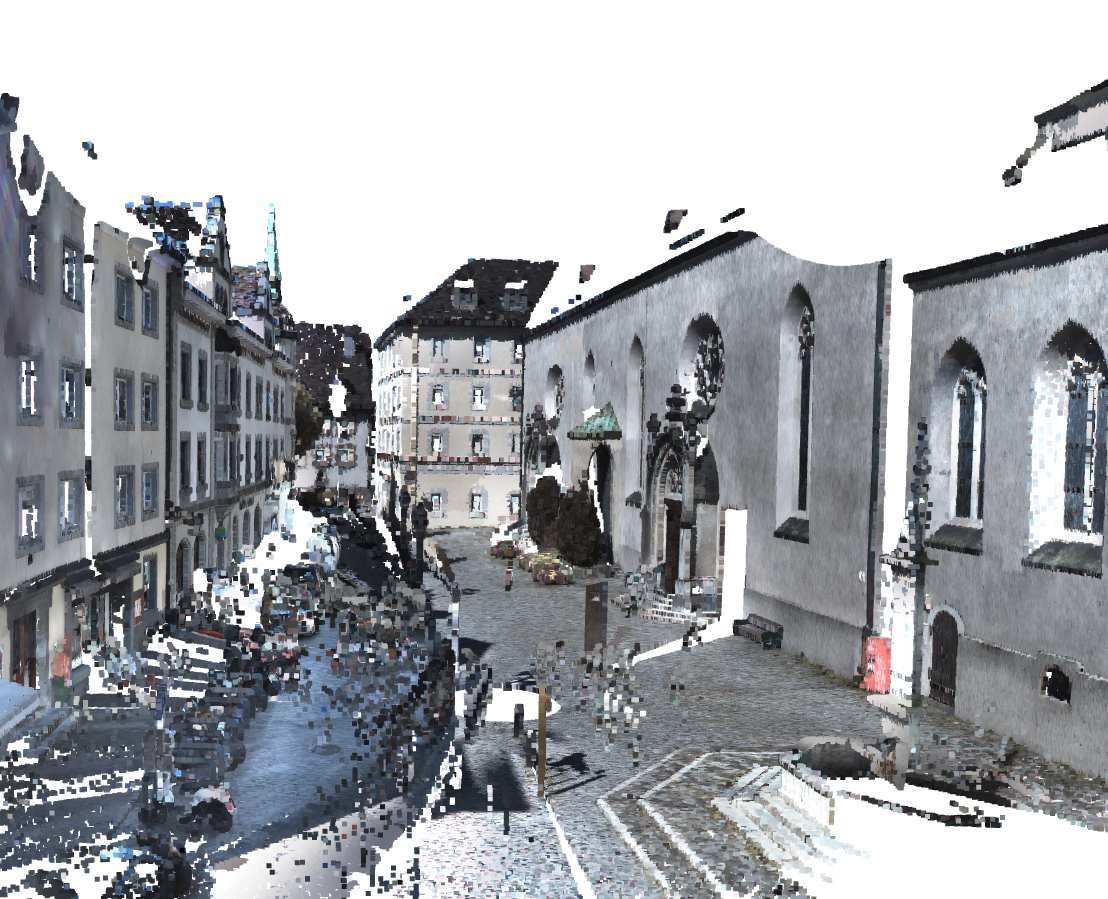
\includegraphics[width=0.35\textwidth, height=0.15\textheight]{images/sem3d_data/4.png} & 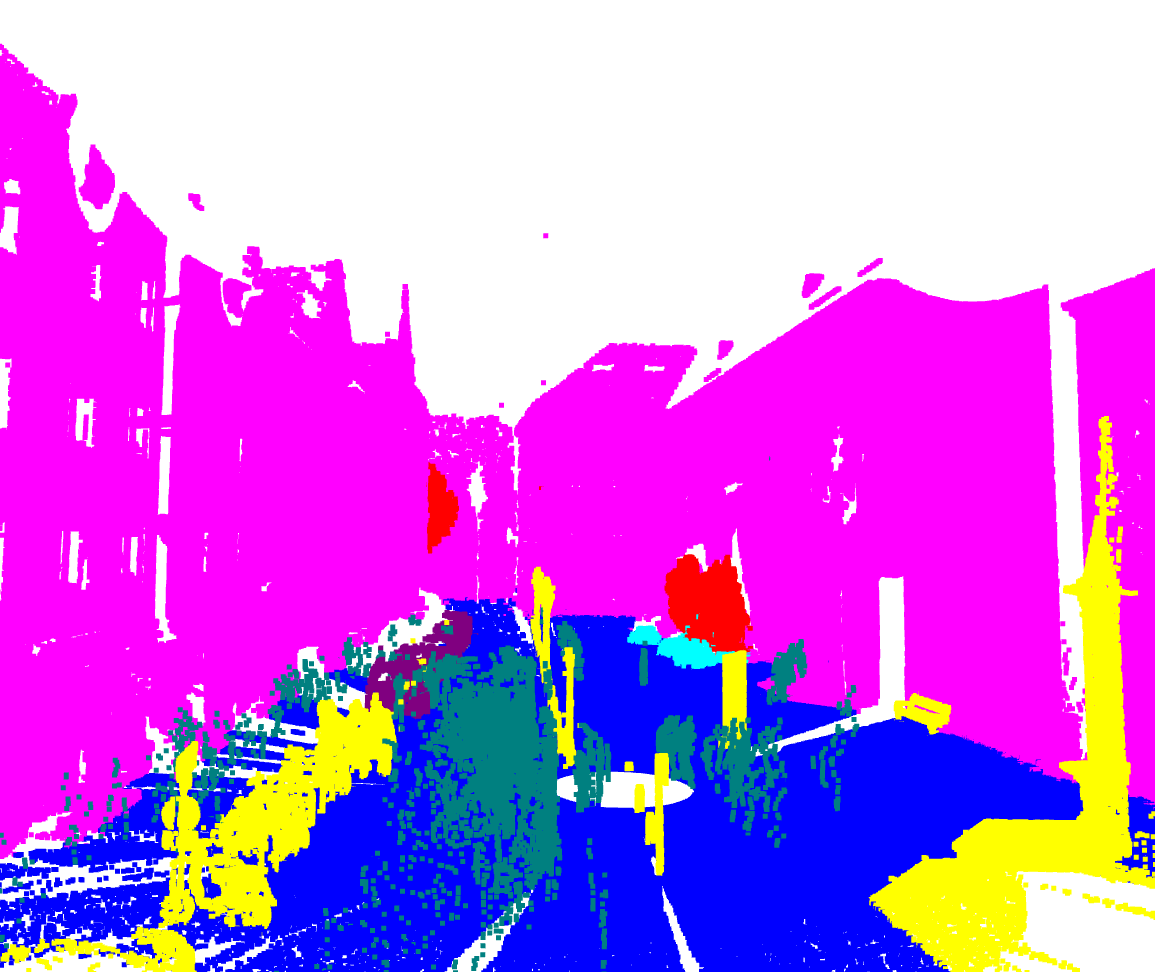
\includegraphics[width=0.35\textwidth, height=0.15\textheight]{images/sem3d_data/4_gt.png}\\
        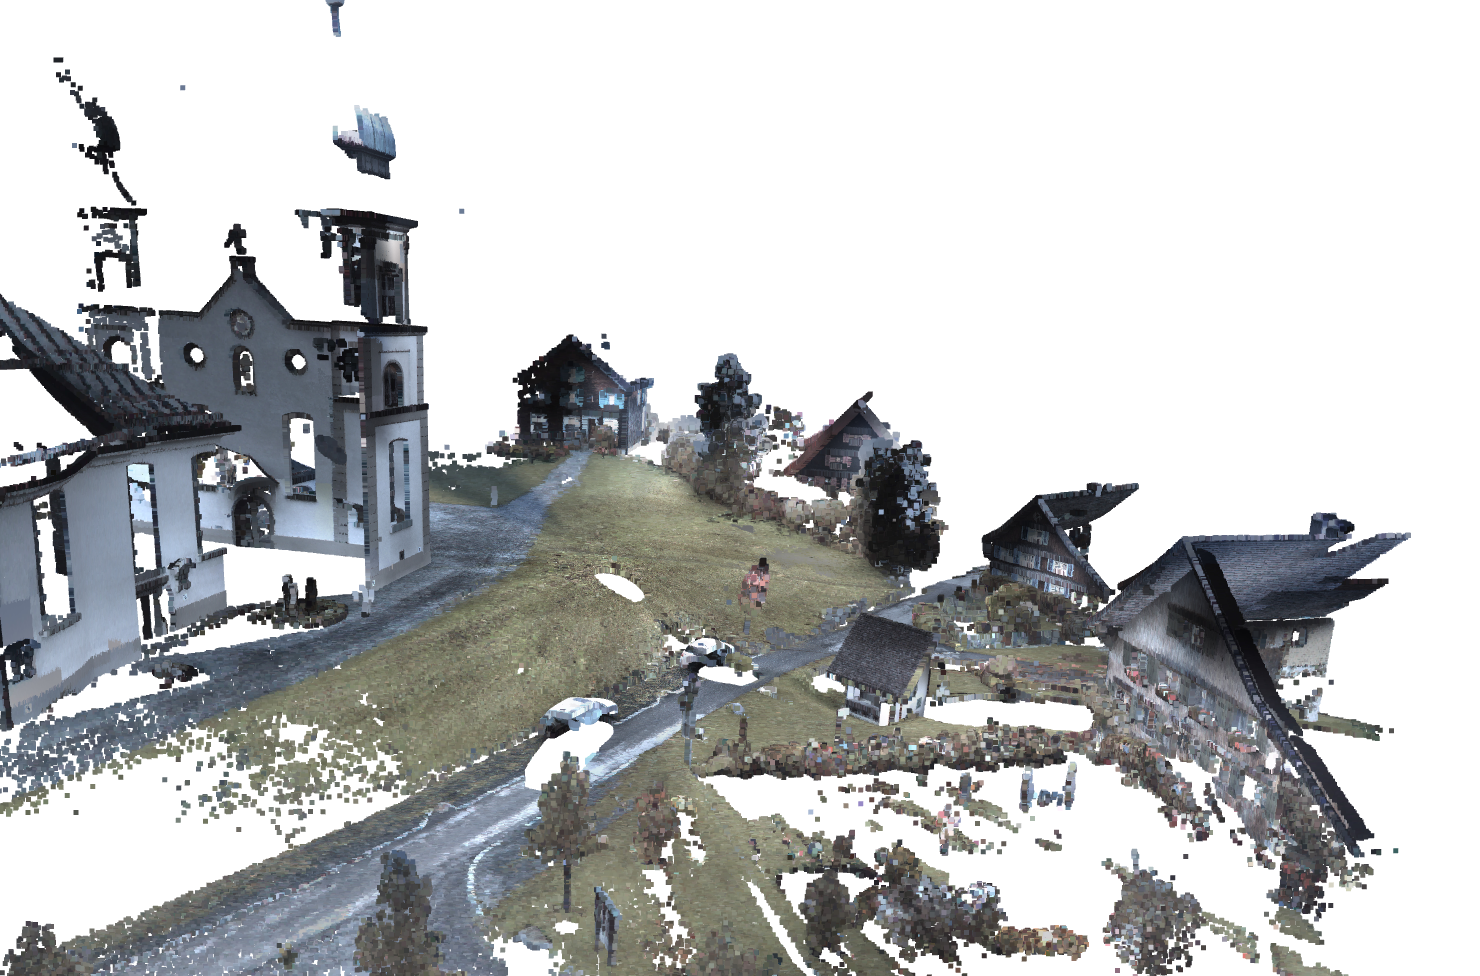
\includegraphics[width=0.35\textwidth, height=0.15\textheight]{images/sem3d_data/5.png} & 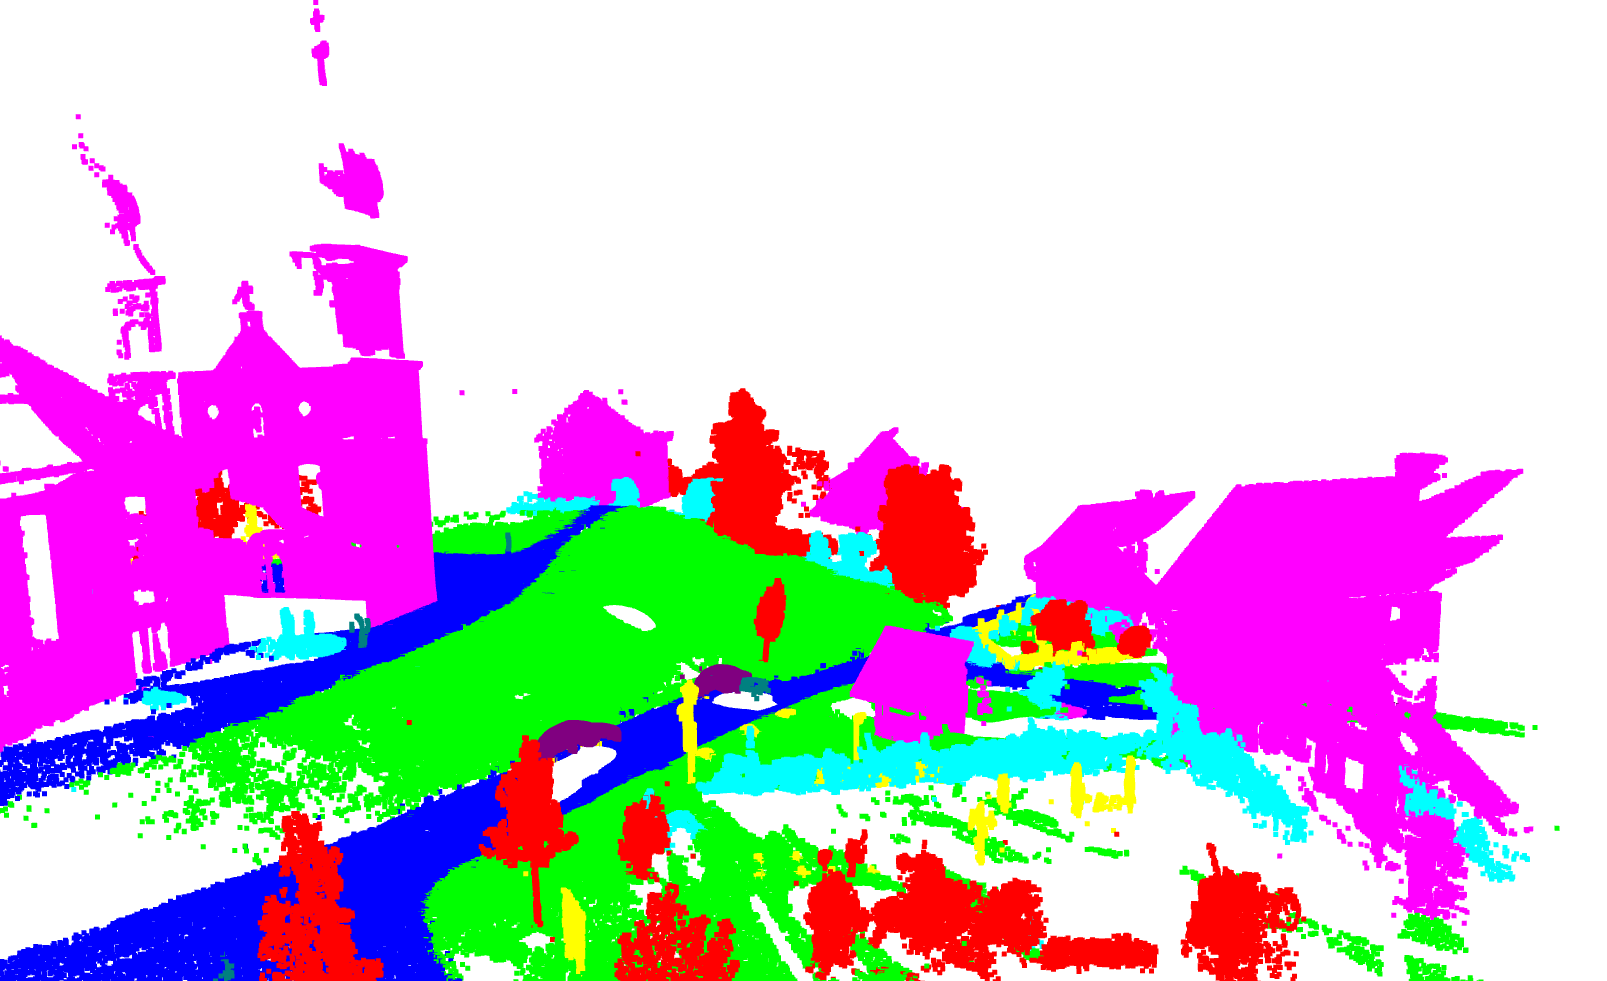
\includegraphics[width=0.35\textwidth, height=0.15\textheight]{images/sem3d_data/5_gt.png}\\
    \end{tabular}
    
\includegraphics[scale=0.65]{images/legend.png}
    \caption{Illustration of point clouds in training and validation set with first column representing RGB colors of point cloud and second columns their ground truth colors with legend given in last image.}
    \label{fig:sem3d_gt_vis}
\end{figure*}
\textcolor{red}{Add how is dataset collected like what kind of sensor they used and its properties.}
\section{S3DIS}
S3DIS is an indoor dataset making it an ideal OOD dataset candidatae becuase of the no class overlap with the Semantic3D dataset.
It is only one of two datasets available in indoor LiDAR dataset candidataes. 
The other is ScanObjectNN whose dataset is not available online.
S3DIS dataset comprises of scans of three different buildings covering an 6020 square meters.
These scans include areas such as personal offices, restrooms, open spaces, lobbies and hallways.
The scans are generated using Matterport 3D scanner \textcolor{red}{add the scan generation technique (mesh to PC)} and can be seen in \textcolor{red}{\textbf{cite figure}}.
S3DIS dataset is divided into 12 classes which are further divided into two subclasses.
\textcolor{red}{Make these classes in points}
First subclass include structural elements which consist of \textit{ceiling, floor, window, wall, beam, columns and door}
and latter subclass has common items such as \textit{table, sofa, chair, board and blackboard}.
Along with ShapeNet dataset \textcolor{red}{cite ShapeNet here}, S3DIS is also one of the most evaluated dataset in indoor setting for semantic segmentation  using in \textcolor{red}{cite S3DIS papers here} whereas ShapeNet is used for part segmentation.

\section{OOD Benchmarking}
In this section we discuss benchmarked datasets and also argue why are they chosen as benchmarking datasets.
We provided two benchmaked datasets one being Semantic3D vs S3DIS and Semantic3D vs Semantic3D (without color).

\textcolor{red}{Future: LIDAR injection like fog}
\subsection{Semantic3D vs S3DIS}
We chose Semantic3D as training (In-Distribution (ID)) dataset because of the following reasons.
Semantic3D is a static dataset which mean high density of points in a scan compared to sequential datasets.
Semantic3D also has RGB colors as input features along with xyz and intensity values.
Having RGB in the dataset helps in differentiating the Out-Of-Distribution (OOD) points from ID points.
Semantic3D has only eight training classes with outdoor scenes this helps in better understanding of each class and also helps in better understanding of the predicitions on OOD dataset.
S3DIS is an indoor dataset, with scans generated in a building.
This difference in scenes (outdoor vs indoor) makes it an ideal dataset benchmark to study.
We expect the Semantic3D trained model to detect S3DIS dataset with relative ease and high confidence because of huge difference in features in scene and visual comparison between these two datasets is shown in Figure~\textcolor{red}{cite}.
\textcolor{red}{Add comparison image here}

\subsection{Semantic3D (color) vs Semantic3D (without color)}
Since our main hypothesis is that RGB colors play a major role in detecting the OOD objects.
So we removed the colors of the Semantic3D dataset and since the model requires RGB values for prediction we changed the color of points to black.
The example visual comparison for this benchmark is depicted in Figure~\textcolor{red}{cite}.
\end{document}